\documentclass{bioinfo}
\copyrightyear{2005}
\pubyear{2005}
\usepackage{graphicx}

\begin{document}
\firstpage{1}

\title[BioPax to SBML qual]{Qualitative translation of relations from BioPax to SBML qual}
\author[B\"uchel \textit{et~al}]{Finja B\"uchel\,$^{1,*}$,
and Andreas Zell\,$^1$\footnote{to whom correspondence should be addressed}}
\address{$^{1}$Department of Cognitive Systems, University of Tuebingen, Sand 1, 72076 T\"ubingen, Germany\\}


\history{Received on XXXXX; revised on XXXXX; accepted on XXXXX}

\editor{Associate Editor: XXXXXXX}

\maketitle

\begin{abstract}

\section{Motivation:}
The goal of systems biology is the modeling and understanding of biological and chemical processes in a cell. Thus, in-silico models are build to reproduced thoses cellular processes. One distinguishes between quantitative and qualitative models. Quantitative models incorporate data which can be quantified numerically. In contrast, qualitative models describe the relationship between the model entities. SBML and BioPax are two of the most popular modeling languages. Until the release of the SBML extension package, SBML qual, it was not possible to describe qualitative models with SBML. That was exclusively possible with BioPax. The BioCarta database includes pathway models which contain both reactions and relations. These models are described with the BioPax format but, up to no, not with the SBML qual format.
\section{Results:}
We provide a complete collection of converted BioCarta pathways in the new SBML qual format. Furthermore, both BioPax level 2 and level 3 pathways are translated.
\section{Availability:}
The complete collection of the BioCarta models is freely available on our homepage ..... (\textbf{TODO Finja: create homepage!})

\section{Contact:} \href{finja.buechel@uni-tuebingen.de}{finja.buechel@uni-tuebingen.de}
\end{abstract}

\section{Introduction}
\begin{itemize}
\item Allgemeines zu Modellen
\item SBML, BioPax sehr g�ngige Formate, die am meisten verwendet werden
\item SBML fr�her nur reaktionen, jetzt mit qual -> a new converter is necessary, that old knowledte isn't lost. or old knowledge can be extended
\item Vorteile von qual
\end{itemize}
\textbf{TODO: Florian und Andreas: Habt ihr hier noch konkrete Ideen, was ich noch einbauen k\"onnte? Stichworte reichen v\"ollig.}


\begin{methods}
\section{Material and Methods}
\subsection{Material BioCarta}
\textbf{TODO: Finja rewrite}
 BioCarta pathways of the nature Pathway Interaction Database (PID) (2). PID provides human pathways in the BioPax format level 3 (3), which specifies for each interaction a ControlType attribute. The ControlType attribute determines if the interaction is activating or inhibiting.
%(2) Carl F. Schaefer, Kira Anthony, Shiva Krupa, Jeffrey Buchoff, Matthew Day, Timo Hannay & Kenneth H. Buetow. PID: The Pathway Interaction Database. Nucleic Acids Res. 37, D674-9 (2009)
%(3) Demir et al. Nature Biotechnology 28 , 935�942 (2010) doi:10.1038/nbt.1666



\subsection{Specification of SBML qual}
\begin{itemize}
\item QualtitativeModel
\item QualitativeSpecies
\item Transition: All interactions between two or more entities, which are not molecular reactions, are named relation. These relations describe enzyme-enzyme relations, protein-protein interactions, interactions of transcription factors and genes, protein-compound interaction and links to other pathways. In SBML, qual describes relations as Transitions. Transitions consist of Input, Output, and Term objects. SBML qual specifies the kind of relation in the variable �sign� of the Input object. The sign variable can have the value �positive�, �negative�, �dual�, and �unkown�. \textbf{TODO Finja: Rewrite, because the same text in path2models}
\item Input
\item Output
\item FunctionTerm \textbf{TODO Florian: K\"onntest du hier bitte ein oder zwei S\"atze schreiben?}
\item Symbol     \textbf{TODO Florian: K\"onntest du hier bitte ein oder zwei S\"atze schreiben?}
\item
\end{itemize}


\subsection{Specification of BioPax level 2 and 3}
\textbf{TODO Finja: Grobe Beschreibung, Verweis auf Publikationen}

\subsection{Conversion of BioPax to SBML qual}
\begin{itemize}
\item Species is determined automatically (if it is mentioned in the file)
\item Works file vice, 1 file = 1 pathway
\item how is distinguished between a transition and a reaction... -> include table
\item annotations of the species? \textbf{TODO Clemens: K\"onntest du das bitte ausf\"uhren/erg\"anzen?SBO terms, GO,...?}
\end{itemize}


\begin{table}[!t]
\processtable{Description of the translation of BioPax control elements\label{Tab:BioPax2SBML}}
{\begin{tabular}{llll}\toprule
BioPax controller & BioPax controlled & Converted\\
                  &                   & SBML qual\\
                  &                   & element\\
\midrule
\textbf{BioPax level 3}\\
\midrule
PhysicalEntity & BiochemicalReaction               & Reaction\\
PhysicalEntity & ComplexAssembly                   & Reaction\\
PhysicalEntity & Control                           & Transition\\
PhysicalEntity & Degradation                       & Transition\\
PhysicalEntity & Transport                         & Transition\\
PhysicalEntity & TransportWithBiochemicalReaction  & Reaction\\
PhysicalEntity & Pathway                           & Transition\\
PhysicalEntity & TemplateReaction                  & Transition\\
\\
Pathway         & BiochemicalReaction               & Transition\\
Pathway         & ComplexAssembly                   & Transition\\
Pathway         & Conversion                        & Transition\\
Pathway         & Degradation                       & Transition\\
Pathway         & Pathway                           & Transition\\
Pathway         & TemplateReaction                  & Transition\\
Pathway         & Transport                         & Transition\\
Pathway         & TransportWithBiochemicalReaction  & Transition\\
\\\midrule
\textbf{BioPax level 2}\\
\midrule
physicalEntity & biochemicalReaction               & Reaction\\
physicalEntity & complexAssembly                   & Reaction\\
physicalEntity & control                           & Transition\\
physicalEntity & pathway                           & Transition\\
physicalEntity & transport                         & Transition\\
physicalEntity & transportWithBiochemicalReaction  & Reaction\\
\\
pathway         & biochemicalReaction               & Transition\\
pathway         & complexAssembly                   & Transition\\
pathway         & conversion                        & Transition\\
pathway         & pathway                           & Transition\\
pathway         & transportWithBiochemicalReaction  & Transition\\
pathway         & transport                         & Transition\\\botrule
\end{tabular}}{BioPax control elements consists of a controller and one or more controlled elements. Depending on the kind of controller or controlled element, a reaction or a transition can be converted to SBML qual. The table gives an overview of this conversion regarding BioPax level 2 and BioPax level 3.}
\end{table}

\subsection{Conversion of BioPax level 2}


\begin{figure*}[!th]
\centering 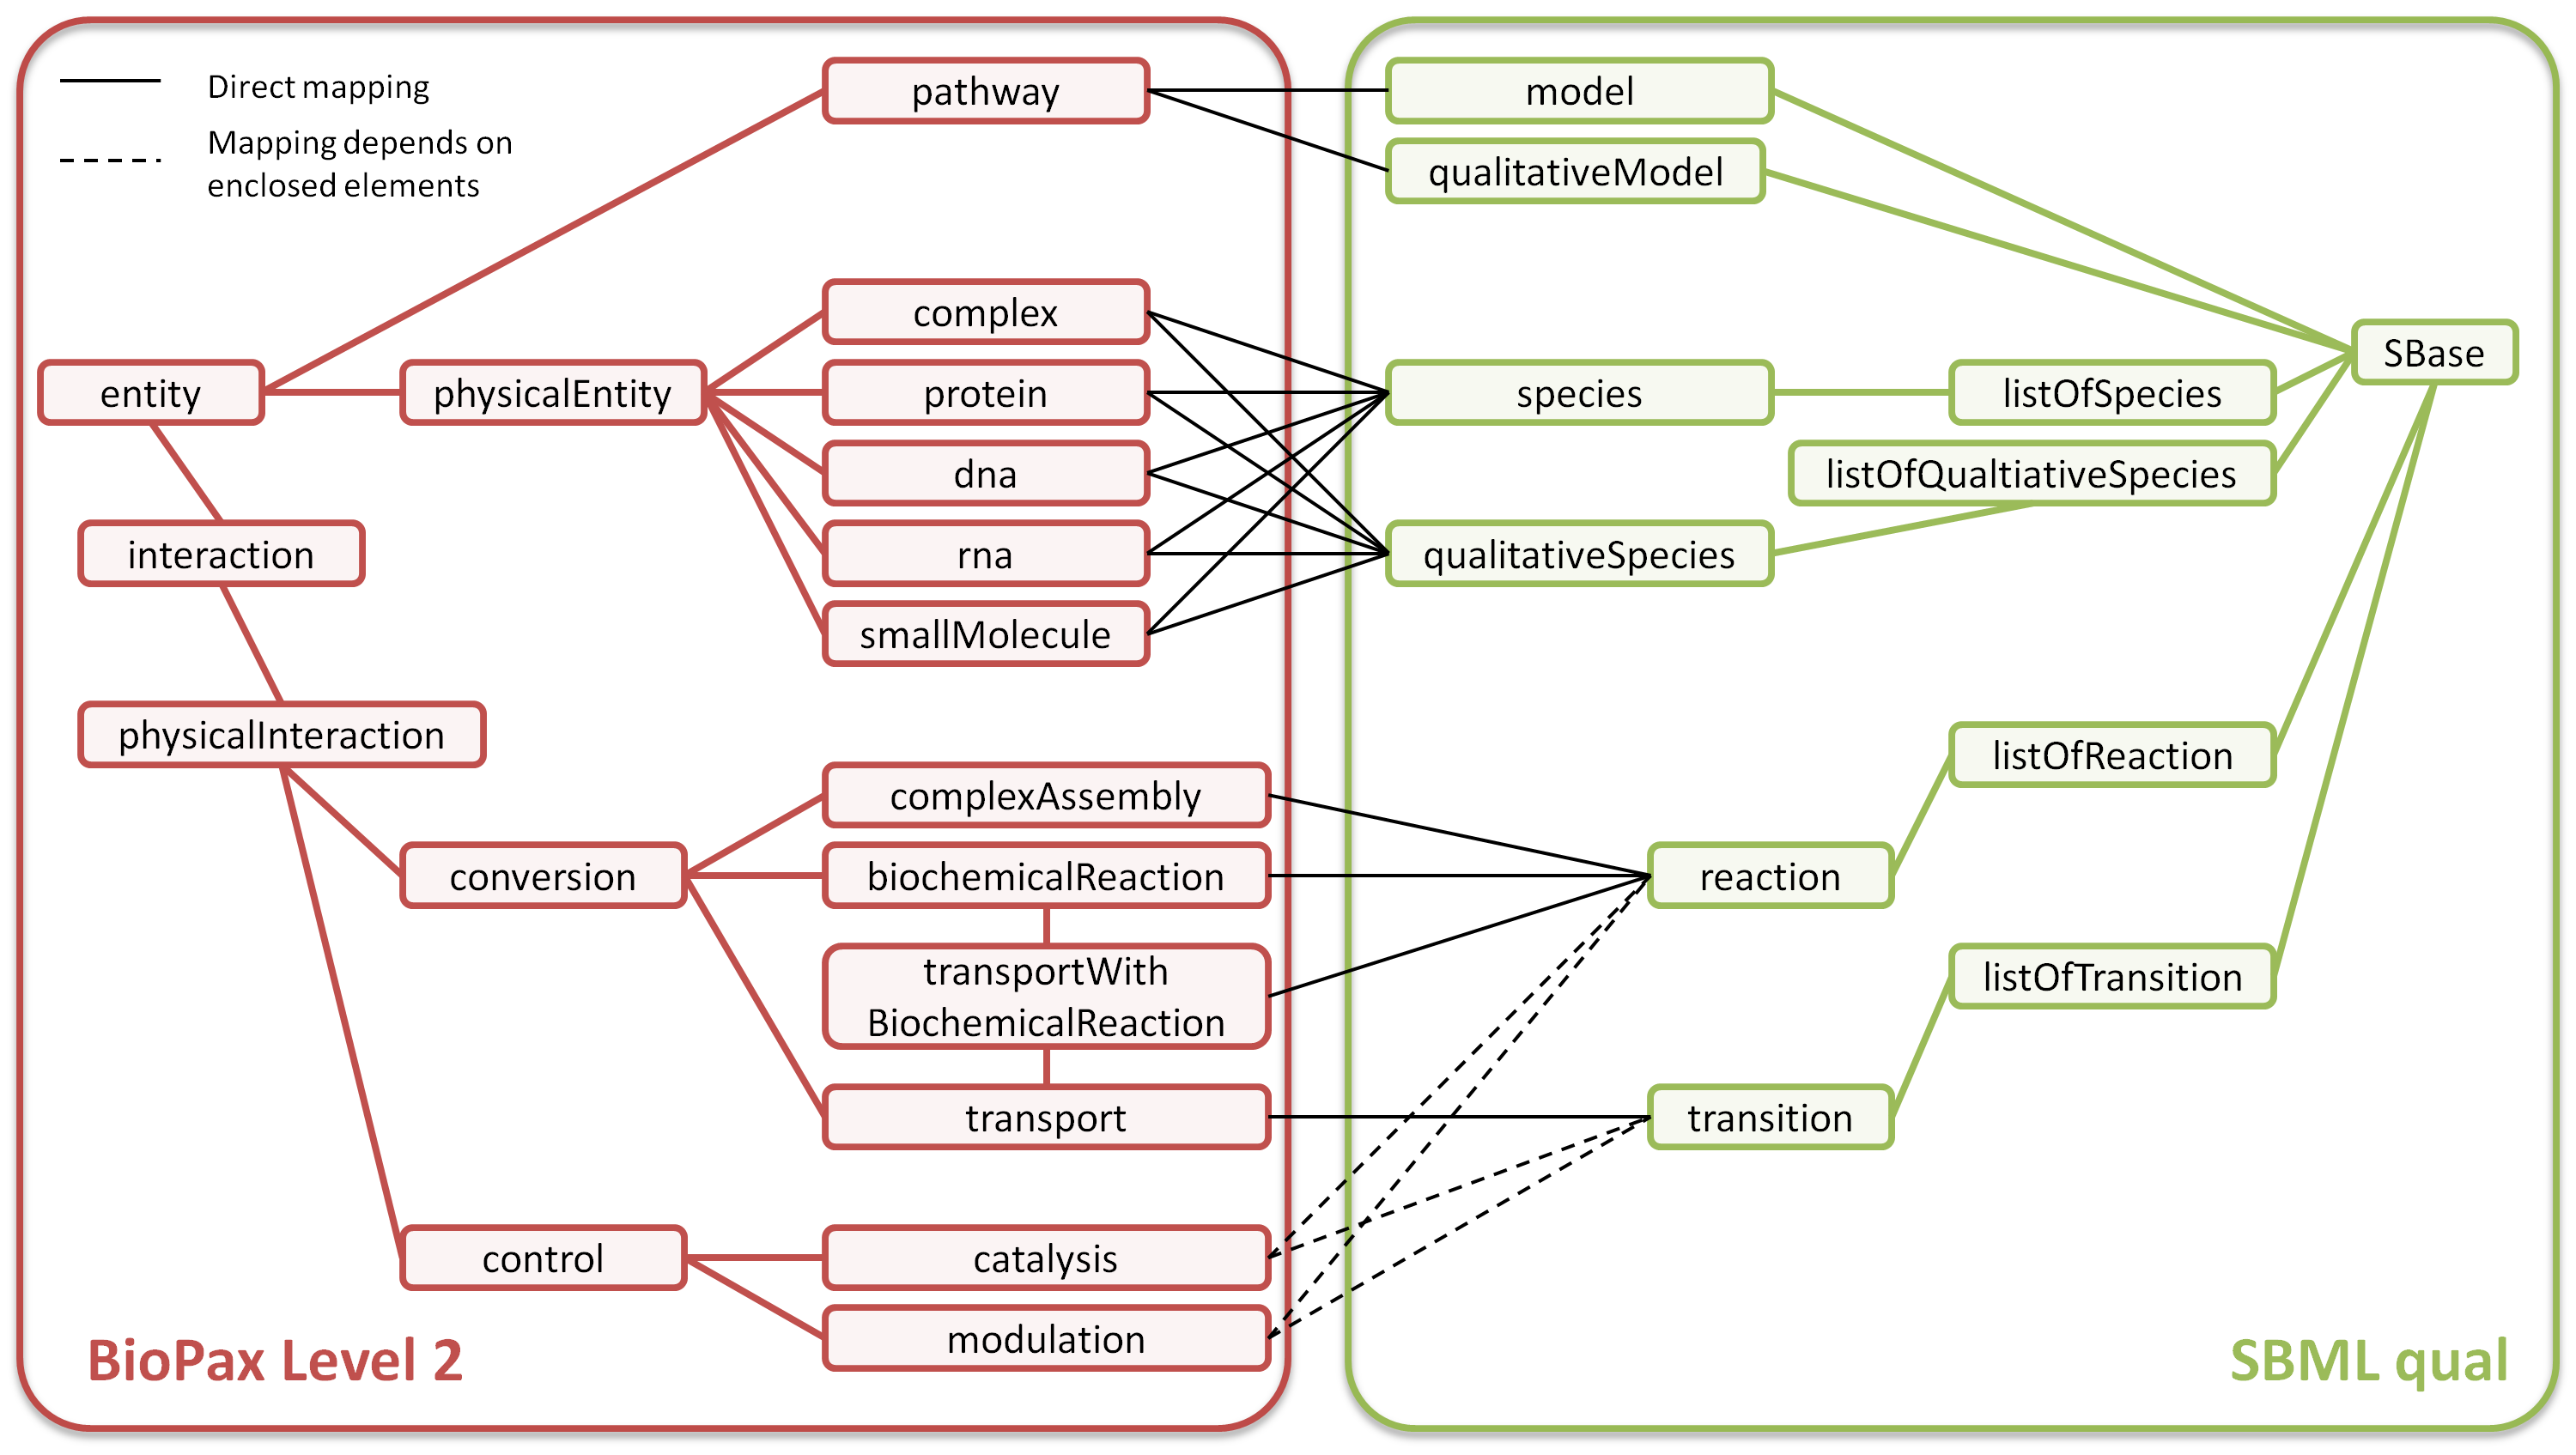
\includegraphics[width=0.96\textwidth]{BioPax2SBMLqual.png}
\caption{Conversion from BioPax Level 2 to SBML qual. The red rounded rectangles and lines describe the BioPax leve 2 elements and how they are inherited. SBML qual entities are colored green. The conversion from BioPax level 2 to SBML qual is colored black.}\label{fig:BioPax2SBMLqual}
\end{figure*}


\subsection{Conversion of BioPax level 3}
\begin{figure*}[!th]
\centering 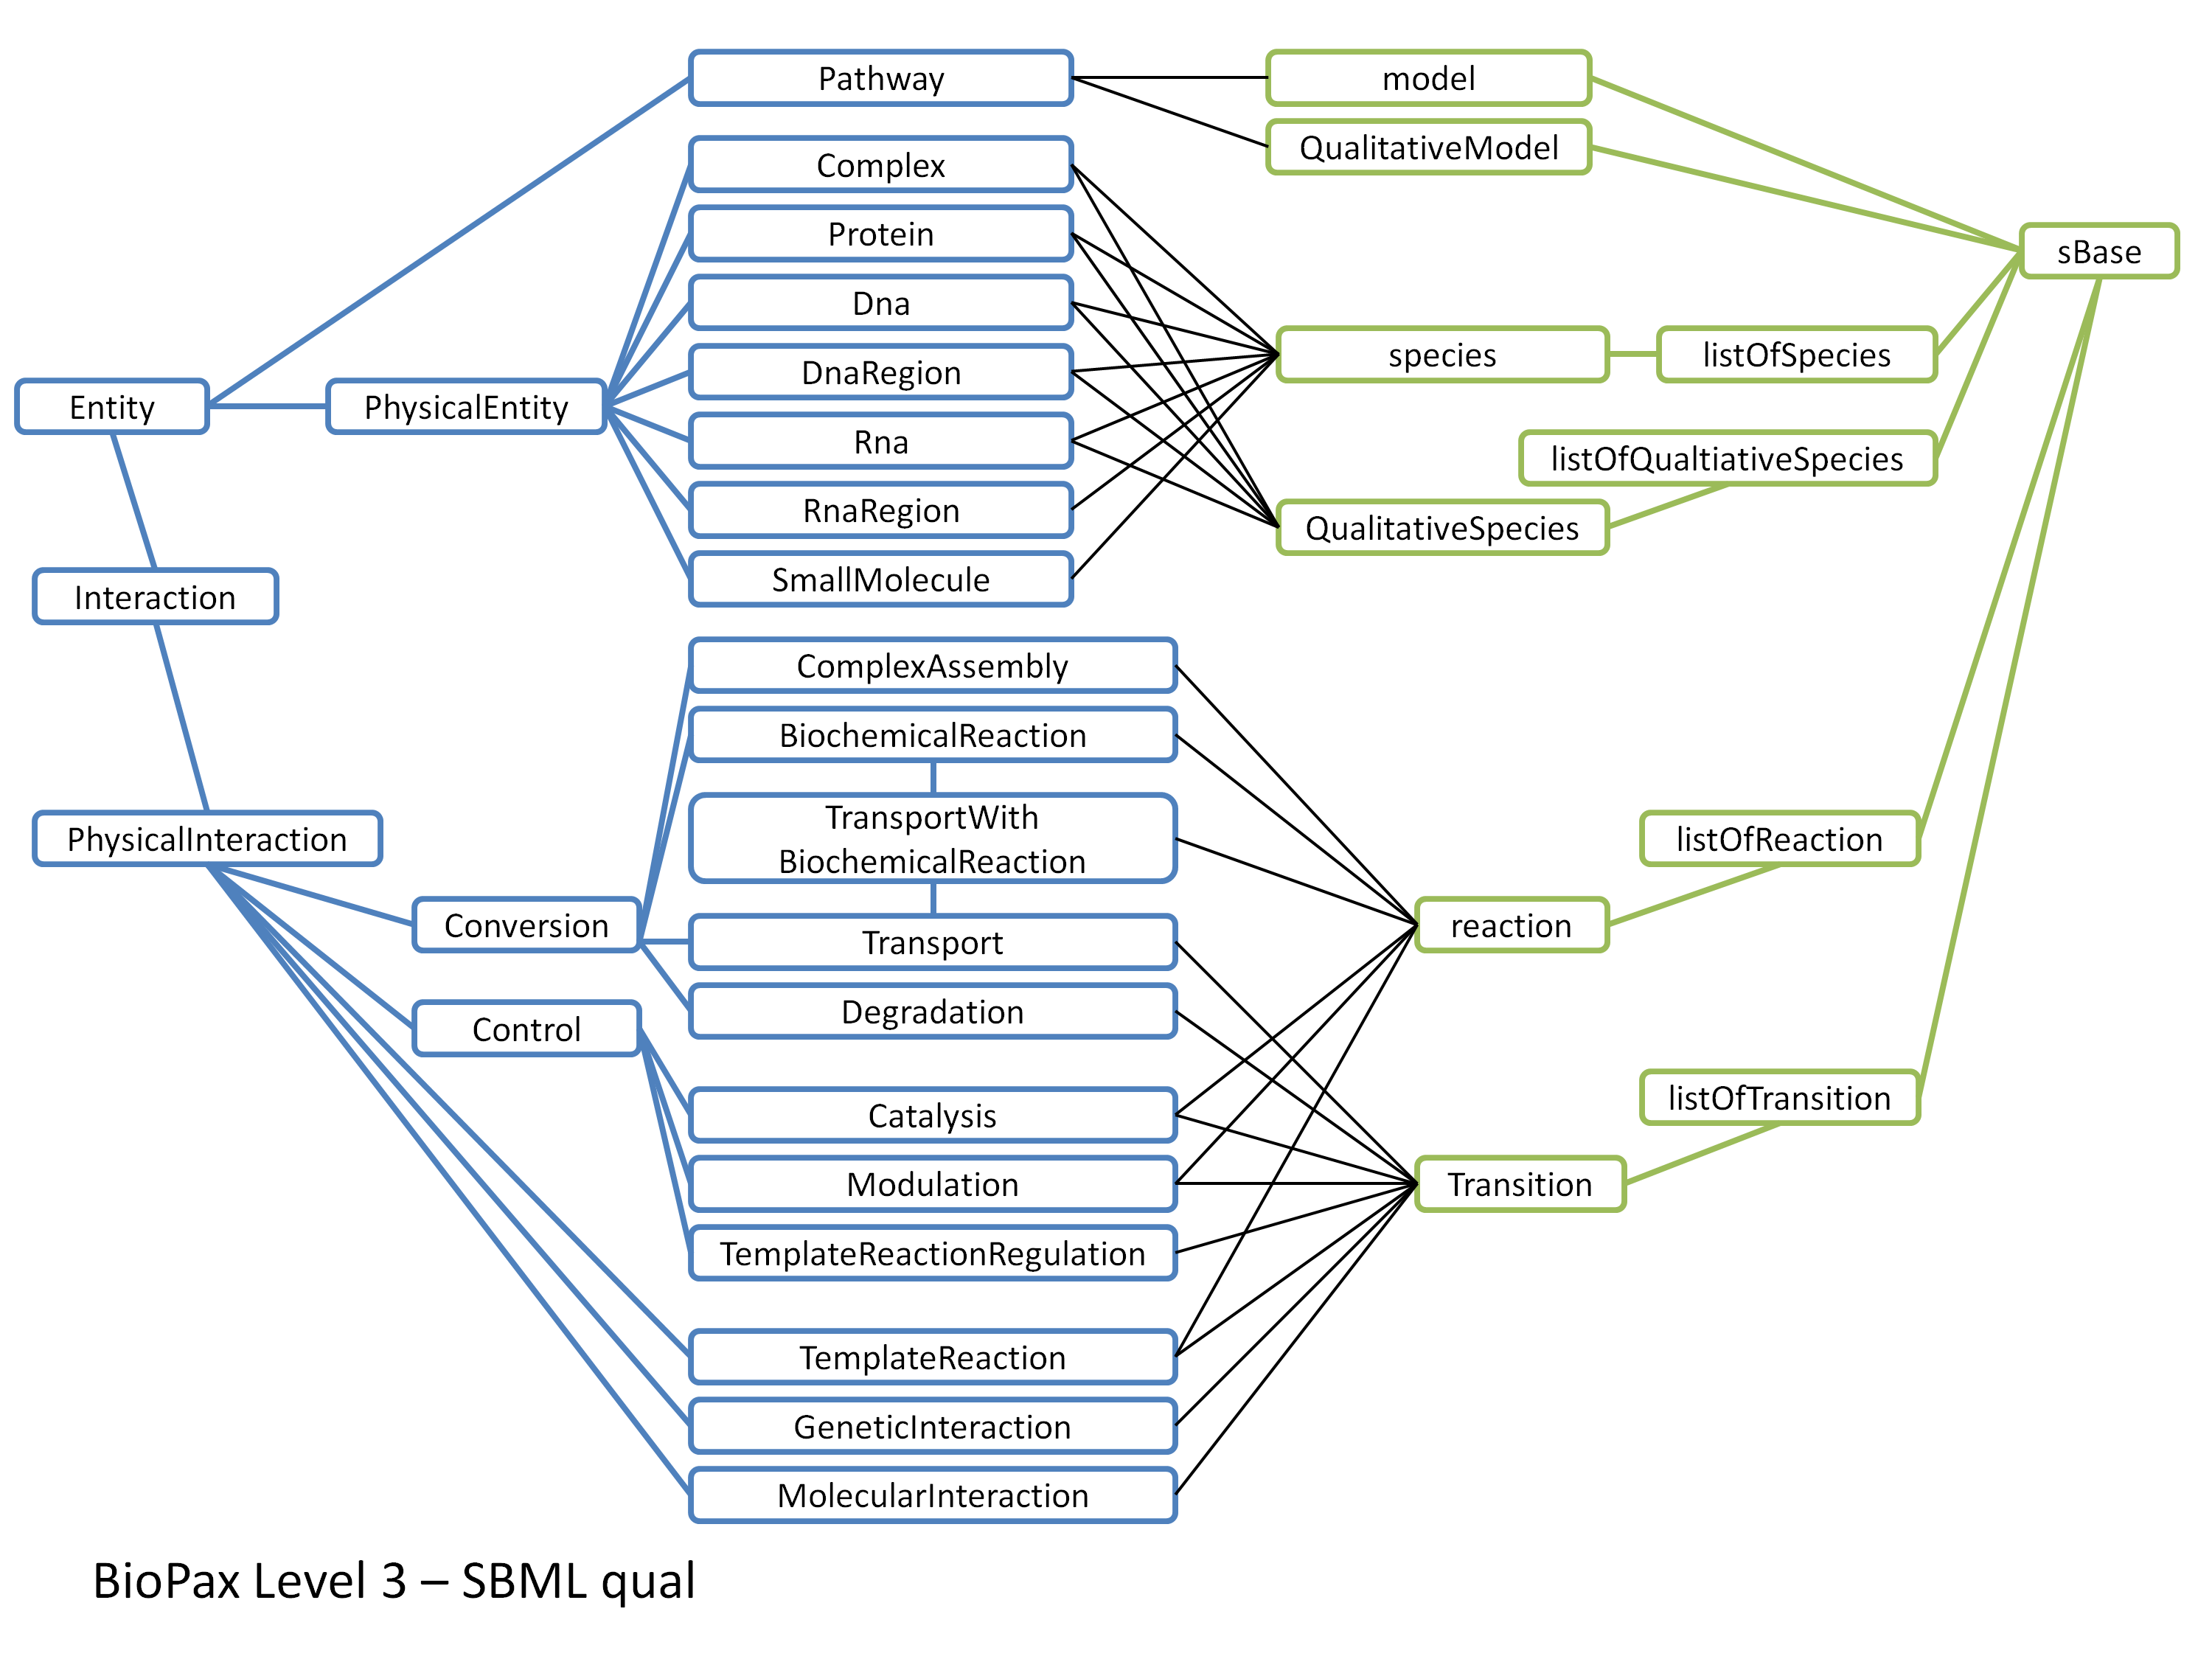
\includegraphics[width=0.96\textwidth]{BioPax3SBMLqual.png}
\caption{Conversion from BioPax Level 3 to SBML qual. The blue rounded rectangles and lines describe the BioPax leve 2 elements and how they are inherited. SBML qual entities are colored green. The conversion from BioPax level 2 to SBML qual is colored black.}\label{fig:BioPax3SBMLqual}
\end{figure*}


\begin{itemize}
\item TODO: Conversion/Control elemente nochmal zus�tzlich einzeichnen?
\end{itemize}
\end{methods}


\section{Results and Discussion}
Warum ist es so toll qual Modelle zu haben

\section{Conclusion}
.....


\section*{Acknowledgement}
We thank xy.

\paragraph{Funding\textcolon} German Federal Ministry of Education and Research (BMBF) [National Genome Research Network (NGFN+) under grant number 01GS08134].

\bibliographystyle{natbib}
%\bibliographystyle{achemnat}
%\bibliographystyle{plainnat}
%\bibliographystyle{abbrv}
%\bibliographystyle{bioinformatics}
%\bibliographystyle{plain}
%
\bibliography{document}

\end{document}
